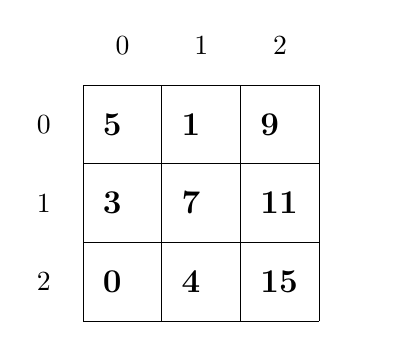
\begin{tikzpicture}
  % draw the grid and the numbers
  \draw (-1,-1) grid (2,2) foreach \i in {0,...,2}{
    (\i-.5,2.5) node{\i} (-1.5,1.5-\i) node{\i}};

  \node[text width=1.5cm] at (0.0,1.5) (A_coord) {\large \textbf{5}};
  \node[text width=1.5cm] at (1.0,1.5) (A_coord) {\large \textbf{1}};
  \node[text width=1.5cm] at (2.0,1.5) (A_coord) {\large \textbf{9}};

  \node[text width=1.5cm] at (0.0,0.5) (A_coord) {\large \textbf{3}};
  \node[text width=1.5cm] at (1.0,0.5) (A_coord) {\large \textbf{7}};
  \node[text width=1.5cm] at (2.0,0.5) (A_coord) {\large \textbf{11}};

  \node[text width=1.5cm] at (0.0,-0.5) (A_coord) {\large \textbf{0}};
  \node[text width=1.5cm] at (1.0,-0.5) (A_coord) {\large \textbf{4}};
  \node[text width=1.5cm] at (2.0,-0.5) (A_coord) {\large \textbf{15}};

\end{tikzpicture}
